% !TeX spellcheck = <none>
% UTF-8 encoding
% Compile with latex+dvipdfmx, pdflatex, xelatex or lualatex
% pdflatex is recommanded 
% This template is released under BSD 2-Clause license.

% xelatex lualatex 无法使用, Package fontspec Error: The font "SimHei" cannot be found. \section*{摘要}
% 经测试,pdflatex 和 latex 是可以使用的,但luatex编译速度极其慢(在windows上)
% 在archlinux上,pdflatex 无法使用,默认字体是fandol系列,没有相应字体,网上的回答是pdflatex不支持中文,但windows里的pdflatex就行
% archlinux上测试,xelatex是可以使用的,只要安装texlive元包和texlive-langchinese就行,texlive元包中有tixlive-fontsextra,基本的字体都有,就是没有fandol
\documentclass[UTF8]{ctexart}
\usepackage{ifpdf,ifxetex,ifluatex}

\ifPDFTeX	
	\pdfoptionpdfminorversion = 7	%  7表示你的PDF版本 % 只有pdflatex可以用这句话,表示输出PDF文件的版本,使用latex时请注释
\fi

\ifXeTeX
	\usepackage{ifplatform}
	\ifwindows
		\errmessage{在windows上请用pdflatex进行编译,xelatex在windows上字体映射好像有问题}
	%\fi %不知道为啥这里不需要这个
\fi


% 自定义的一些颜色
\usepackage{xcolor}
\definecolor{hyperref-green}{RGB}{0,150,0}
\definecolor{hyperref-red}{RGB}{200,0,0}
\definecolor{hyperref-blue}{RGB}{0,0,200}
\definecolor{hyperref-black}{RGB}{0,0,0}
% 超链接
\usepackage[
    citecolor=hyperref-black,
    linkcolor=hyperref-black,
    urlcolor=hyperref-black,
    menucolor=black,
    breaklinks=true,
    bookmarks=true,
    colorlinks
]{hyperref}

%\usepackage{bibentry} % 可以将参考文献条目编排在文本的任何位置,常用于创建附有评注的参考文献
%导入外部pdf
\usepackage{pdfpages} % includepdf

%% 公式和数学标识相关%%%%%%%%%%%%%%%%%%%%%%%%%%%%%%%%%%%%%%%%%%%%%%%%%
\usepackage{amsmath}
\usepackage{bm} %%某些矢量需要加粗字符,除mathbf外的另一种方式%By Kuber
\usepackage{amssymb}
\usepackage{pifont} %提供了一些符号和图案,如圆圈数字、箭头、星星、钩子等等
\usepackage{listings} %插入代码
\usepackage[ruled]{algorithm2e} %算法和伪代码
\newcommand{\cmark}{\checkmark}%
\newcommand{\xmark}{\ding{55}}%

\usepackage{diagbox} %为空单元格绘制斜表线
\numberwithin{equation}{section} % 公式按章节编号
\numberwithin{table}{section} % 公式按章节编号

\usepackage{amsfonts}
%%%%%%%%%%%%%%%%%%%%%%%%%%%%%%%%%%%%%%%%%%%%%%%%%%%%%%%%%%%%%%%%%%

% 插入图表和图表描述
\usepackage{graphicx, caption, subfigure, float}
\DeclareCaptionFormat{myformat}{\zihao{5}\selectfont#1#2#3} % 标题 5号字体 
\captionsetup{format=myformat}
\setlength{\abovecaptionskip}{0pt} % 设置标题与上文之间的间距
\setlength{\belowcaptionskip}{-10pt} % 设置标题与下文之间的间距
\captionsetup{justification=centering} %标题居中
\usepackage{overpic} % 在图上插入图片或公式
\usepackage{pgfplots} % 绘图

%====================================================
% 其他格式,和样式
% 将章节标号转为中文
\usepackage{zhnumber}
%% geometry
\usepackage{geometry}
\geometry{left=3.17cm,right=3.17cm,top=3.0cm,bottom=3.0cm}  % 页边距

% 页眉相关的设置
\usepackage{fancyhdr}

%%%%%%%%%%%%%%%%%%%%%%%%%%%%%%%%%%%%%%%%%%%%%%%%%%%%%%%%%%%%%%%%%%%%%%%%%%%%%
% cqzw555 添加的包
\usepackage[list=off]{bicaption} % 在 figure 或者 table 环境中使用 \bicaption 命令生成中英文双语标题,list=off代表插图索引表中不出现英文标题
\captionsetup[figure][bi-second]{name=Figure} %设置图的英文编号前缀
\captionsetup[table][bi-second]{name=Table} %设置表的英文编号前缀
\usepackage{newtxtext} % 提供文本的Times New Roman
% \usepackage{tablefootnote} % 表格脚注
\usepackage{comment} %注释

% 使用bibtex作为默认文献工具则可以使用gbt7714包,但因为没有找到合适样式而改成biblatex
%\usepackage{natbib} % biblatex 和 natbib 不兼容,而 gbt7714 和 natbib 是兼容的
%\usepackage[sort&compress]{gbt7714} %GBT7714文献引用格式
%\bibliographystyle{gbt7714-numerical}
\usepackage[backend=biber, style=gb7714-2015]{biblatex} % biblatex
% 使用biblatex时需要将texstudio中默文献工具改为biber,默认编译器改为pdflatex
% texlive(2023) 中基于 biblatex 实现的 gb7714 有多个样式,分别如下
%   标准版gb7714: gb7714-2015,gb7714-2005,gb7714-1987
%   按照author,year顺序进行引用的:gb7714-2015ay,gb7714-2005ay
%   按照引用顺序进行引用的:gb7714-2015ms
%   numerical sequence and authoryear mixed style:gb7714-2015mx
%   华中师范大学:gb7714-CCNU
%   西北农林:gb7714-NWAFU
%   东南大学:gb7714-SEU
% 不同样式的效果自行尝试

%这个来自华中师范的样式,关键是lowercase
\ExecuteBibliographyOptions{
	gbpunctin    = false,
	gbfieldtype  = false,       % 输出type域,主要处理学位论文,true在学位论文的[D]后面打印硕士学位论文
	gbnamefmt=lowercase % 这应该是控制名字首字母大写的
}

% 没有明确看到这个间距的要求,但看到张喆的间距比我大,把这个设置项添上,以后可能有用
\setlength{\biblabelsep}{1em} % 设置标签到参考文献内容的间距

% 以下这部分来自西北农林,控制参考文献字号
\newcommand\nwafubibfont{\zihao{-4}}% 字体
\renewcommand{\bibfont}{\nwafubibfont}% 全局字体设置

% biblatex 里要求的设置文献库文件的方式
\addbibresource{master-thesis.bib}
\usepackage{color}
\usepackage{booktabs} % for cmd 'toprule', 'bottomrule'
\usepackage{multirow} % for cmd 'multirow', 'multicolumn'
\usepackage{enumitem}
\usepackage{todonotes}
%\renewcommand{\algorithmcfname}{算法-}  %<---细节与重点
%\SetKwInput{KwIn}{输入}  %<---细节与重点
%\SetKwInput{KwOut}{输出}  %<---细节与重点
% 设置目录格式
\usepackage{titletoc}
\usepackage{titlesec}
%设置目录格式
%\titlecontents{标题名}[左间距]{标题格式}{标题标志}{无序号标题}{指引线与页码}[下间距]
\titlecontents{section}[0cm]{\zihao{-4}\bfseries\filright}{\textbf{\thecontentslabel}\quad}
{}{\textmd{\titlerule*[3pt]{.}\contentspage}}
% 目录中section标题和序号需要加粗,但指引线和页码不加粗,因此在页码和指引线这里用\textmd让文字回到正常状态
\titlecontents{subsection}[0.37cm]{\zihao{-4}\filright}{\contentspush{\thecontentslabel}\quad}
{}{\titlerule*[3pt]{.}\contentspage}
\titlecontents{subsubsection}[0.74cm]{\zihao{-4}\filright}{\contentspush{\thecontentslabel}\quad}
{}{\titlerule*[3pt]{.}\contentspage}

% 目录标题为黑体小二,居中对齐;目录内容全为小四号,中文用黑体,英文用Times New Roman,省略号和数字用等线,左端对齐,一级标题置顶并加粗,
% 其余标题首行缩进0.37 厘米。目录的标题和内容的段前、段后均为0

% 设置标题格式
\ctexset{
	section={
		format+=\heiti\zihao{-2}\centering,  % 定义标题样式,居中对齐
		name={第,章},
		number={\chinese{section}},  % 定义标题的标签,即标题的标号
		aftername=\quad,   % 定义标题和标号之间的水平距离
		beforeskip=24pt,  %段前 24磅
		afterskip=18pt  %断后 18磅
	},
	subsection={
		format+=\heiti\zihao{-3}\raggedright,
		name={},
		number={\arabic{section}.\arabic{subsection}},
		aftername=\quad,
		beforeskip=24pt,  %段前 24磅
		afterskip=18pt  %断后 18磅
	},
	subsubsection={
		format+=\heiti\zihao{4}\raggedright,
		name={},
		number={\arabic{section}.\arabic{subsection}.\arabic{subsubsection}},
		aftername=\quad,
		beforeskip=12pt, %段前 12磅
		afterskip=6pt %段后 6磅
	}
}  %设置标题格式

\ctexset{%
	contentsname={目\hspace{\ccwd}录},
	listfigurename={插图索引},
	listtablename={表格索引},
	figurename={图},
	tablename={表},
	bibname={参考文献},
}

% \usepackage{ulem} % 删除线 \sout
% cqzw555 添加的包 ending

\setlength{\headheight}{12.64723pt}
\addtolength{\topmargin}{-0.64723pt}
%%%%%%%%%%%%%%%%%%%%%%%%%%%%%%%%%%%%%%%%%%%%%%%%%%%%%%%%%%%%%%%%%%%%%%%%%%%%%

\fancyhf{}  % 清除默认页眉
\pagestyle{fancy}
\lhead{上海大学专业硕士学位论文}  % 添加右侧页眉,专硕
%\lhead{上海大学硕士学位论文}  % 添加右侧页眉,学硕
\cfoot{\thepage}  % 添加页脚页码


% 图表按章节编号
\usepackage{chngcntr}
\counterwithin{figure}{section}

%%%%%%%%%%%%%%%%%%%%%%%%%%%%%%%%%%%%%%%%%%%%%%%%%%%%%%%%%%%%%
%常用的命令
\newcommand{\red}[1]{{\textcolor{red}{#1}}} % 把一段字标红
%%%%%%%%%%%%%%%%%%%%%%%%%%%%%%%%%%%%%%%%%%%%%%%%%%%%%%%%%%%%%
% 声明argmin和argmax运算符
\newcommand{\argmin}{\mathop{\mathrm{argmin}}\limits}
\newcommand{\argmax}{\mathop{\mathrm{argmax}}\limits}

% 开始正文
\begin{document}
% 正文格式设置

\zihao{-4} % 小四 字体默认宋体
%\linespread{1.5} \selectfont  % 调整全文为1.4倍line间距,非常接近word版本1.5行间距%By Kuber
\linespread{1.64} \selectfont  % 将行距优化为1.64倍间距
% 目录之后的页码是大写罗马数字
%\begin{comment}

\includepdf[pages={1-5}]{Professional-Master.pdf} % 专硕的封面
% 
\includepdf[pages={1-5}]{cover.pdf} % 学硕的封面
\pagenumbering{Roman} %页码 罗马字母
\setcounter{page}{1}  % LaTeX的起始页码

% !TeX encoding = UTF-8
% !TeX spellcheck = <none>
\section*{摘\hspace{\ccwd}要}
\addcontentsline{toc}{section}{摘要}

硕博士学位论文是研究生从事科研工作成果的主要体现。它能够集中表明学位申请者在研究工作中获得的新发明、理论或见解,是研究生申请硕士或博士学位的重要依据,也是科研领域中的重要文献资料和社会的宝贵财富。
摘要需作者简要介绍本论文的主要内容,主要为本人所完成的工作和创新点。
注:摘要的撰写应符合GB/T 7713.1-2006 的规定。摘要应具有独立性和自含性,即不阅读论文的全文,就能获得必要的信息。摘要的内容应包含与论文等同量的主要信息,供读者确定有无必要阅读全文,也可供二次文献采用。摘要一般应说明研究工作的目的、方法、结果和结论等,重点是结果和结论。摘要中应尽量避免采用图、表、化学结构式、非公知公用的符号和术语。


\vspace{12bp}
\noindent\textbf{关键词:}学位论文;论文格式;规范化;模板

\pagebreak
\section*{ABSTRACT}
\addcontentsline{toc}{section}{ABSTRACT}

Master and doctoral dissertations are the main embodiment of postgraduates engaged in scientific research. It can centrally indicate the new inventions, theories, or insights obtained by degree applicants in their research work. It is an important basis for graduate students to apply for master's or doctor's degree, and also an important literature in the field of scientific research and valuable wealth of society.
The abstract requires author to briefly introduce the main content of dissertation, mainly for the author’s own work and innovation.  
Note: The abstract should be written in accordance with the provisions of GB/T 7713.1-2006. It should be independent and self-contained, that is, necessary information can be obtained without reading the full text. Abstract content should contain the same amount of main information as the dissertation, so that readers can determine whether it is necessary to read the full text, and it can also be used for secondary literature. The abstract should generally describe the purpose, methods, results and conclusions of research work, focusing on the results and conclusions. And try to avoid using figures, tables, chemical structural formulas, non-public symbols and terminology.


\vspace{12bp}
\noindent\textbf{Keywords}:\enskip Dissertation; Dissertation format; Standardization; Template


\pagebreak 

% 由于目录(TOC: table of contents)也会被hyperref作为超链接,因此颜色会被设置为和图表超链接一样的红色,红色的目录不好看。
% 这里单独把TOC的颜色设置为黑色。
{\hypersetup{linkcolor=black}\tableofcontents}
%\end{comment}

%%%%%%%%%%%%%%%%%%%%%%%%%%%%%%%%%%%%%%%%%%%%%%%%%%%%%%%%%%%%%%%%%%%%%%%%%%%%%%%%%%%
%%%%%%%%%%%%%%%%%%%%%%%%%%%%%%%%%%%%%%%%%%%%%%%%%%%%%%%%%%%%%%%%%%%%%%%%%%%%%%%%%%%
% 绪论
\pagebreak
\pagenumbering{arabic}
\setcounter{page}{1}  % LaTeX的起始页码
% !TeX encoding = UTF-8
% !TeX spellcheck = <none>
\section{说明}

Keep it Simple and Stupid !

本模板在\href{https://github.com/zeakey/shu-thesis}{zeakey}的基础上进行创建,并进行了一些修改。修改内容如下:
\begin{enumerate}
	\item 文献管理工具从bibtex改成biber,并使用biblatex包。在使用bibtex时无法将参考文献中作者名从全大写改为首字符大写,放弃使用bibtex
	
	\item 根据今年的上大模板改了目录格式和标题格式。尽管论文模板里是全大写,但在预答辩时,老师提出了这个首字母大写的修改意见,应该是学院的要求不一样。
	
	\item 更近了论文模板,增加专硕论文模板。
	
	\item 增加图片和表格的英文标题支持。现在图片和表格可以增加英文标题了,用法为: $\backslash$bicaption\{中文标题\}\{英文标题\},只要替换原本的caption命令即可。
	
	\item 增加了图片列表和表格列表,不显示英文的图片标题和表格标题。
	
	\item 根据word模板修改了行距
\end{enumerate}

所有的修改全在主tex文件中,所有修改内容都有注释,方便自行调节。
\href{https://github.com/BlueFisher/shuthesis}{BlueFisher}
另外一个上海大学研究生论文模板是\href{https://github.com/BlueFisher/shuthesis}{BlueFisher},这个模板可以自行构建封面,会更方便。我当时只找到这个模板,后续因目录格式等小问题而继续使用源模板。





%
\pagebreak
% !TeX spellcheck = <none>
\section{公式}

便快捷的公式输入是\LaTeX相比于Word的主要优势之一,在熟练掌握的情况下
公式输入的效率会有很大提升。

\LaTeX中的公式主要分为两类:\red{行内公式}和\red{行间公式}。
这是一个行内公式$f(x) = \frac{1}{\sqrt{2\pi}\sigma}\exp{(-\frac{(x-\mu)^2}{2\sigma^2})}$。下面是一个行间公式:
$$
f(x) = \frac{1}{\sqrt{2\pi}\sigma}\exp{(-\frac{(x-\mu)^2}{2\sigma^2})}
$$
这是一个带有编号的公式:
\begin{equation}
	f(x)= |x| = 
	\begin{cases}
		x,& \text{if } x\geq 0\\
		-x,              & \text{otherwise}
	\end{cases}
	\label{eq:cases}
\end{equation}
多行连等公式:
\begin{equation}
	\begin{split}
		f(x) &= |x| \\
		&= \begin{cases}
			x,& \text{if } x\geq 0\\
			-x,              & \text{otherwise}
		\end{cases}
	\end{split}
\end{equation}
带有矩阵的公式:
\begin{equation}
	\mathbf{H} = -\mathbf\mu \cdot \mathbf{B} = -\gamma B_o \mathbf{S}_z = -\frac{\gamma B_o\hbar}{2} 
	\begin{bmatrix}
		1& \cdots &1\\ 
		\vdots & \ddots & \vdots \\
		1 & \cdots & 1 
	\end{bmatrix}.
	\label{eq:matrix}
\end{equation}
带有矢量的公式:%By Kuber
\begin{equation}
	\label{eq:current_density_inandout}
	\bm{J_i} = -\sigma_i \nabla \phi_i ~;~ \bm{J_e}= -\sigma_e \nabla \phi_e ~.
\end{equation}
带有联立大括号的公式:%By Kuber
\begin{equation}
	\label{eq:runge_p_eq}
	\left\lbrace
	\begin{aligned}
		V_{i+1} &= V_i + c_1 K_1 + c_2 K_2 + \cdots + c_p K_p \\
		K_1 &= \Delta t f(t_i ,V_i) \\
		K_2 &= \Delta t f\left(t_i + a_2 \Delta t, V_i + b_{21} K_1\right) \\
		\cdots&~\cdots~\cdots~\cdots~\cdots~\cdots \\
		K_p &= \Delta t f\left( t_i + a_p \Delta t, V_i + b_{p1} K_1 + \cdots + b_{p,p-1} K_{p-1}\right) ~.
	\end{aligned}
	\right.
\end{equation}
对于一个神经网络的求解问题可以公式化成以下形式:
\begin{equation}
	\Theta = \argmin_{\theta} J(\theta)
	\label{eq:argmin}
\end{equation}
式\ref{eq:argmin}中$\Theta$为求得的最佳参数,$\theta$为神经网络的参数,$J(\theta)$为误差函数。

公式可以添加label属性,并在后文中引用。比如公式~\ref{eq:matrix}就可以被引用,
而且点击引用号可以迅速跳转,详情请见第\ref{sec:ref}章。


\pagebreak
% !TeX encoding = UTF-8
% !TeX spellcheck = <none>
\section{算法和伪代码}
%%%%%%%%%%%%%%%%%%%%%%%%%%%%%%%%%%%%%%%%%%%%%%%%%%%%%%%
有时候我们需要在论文中插入一些代码片段来详细说明算法的步骤,
或者需要插入一个伪代码片段来说明算法的流程。

\subsection{插入代码}
% 设置代码样式(关键词颜色,背景颜色,插入代码语言等等)
\lstdefinestyle{customc}{
	belowcaptionskip=1\baselineskip,
	breaklines=true,
	frame=L,
	xleftmargin=\parindent,
	language=C,
	showstringspaces=false,
	basicstyle=\footnotesize\ttfamily,
	keywordstyle=\bfseries\color{green!40!black},
	commentstyle=\itshape\color{purple!40!black},
	identifierstyle=\color{blue},
	stringstyle=\color{orange},
	numbers=left,
}
\lstdefinestyle{customasm}{
	belowcaptionskip=1\baselineskip,
	frame=L,
	xleftmargin=\parindent,
	language=[x86masm]Assembler,
	basicstyle=\footnotesize\ttfamily,
	commentstyle=\itshape\color{purple!40!black},
}
% 插入c语言代码
\lstset{escapechar=@,style=customc}

\begin{lstlisting}[caption={一段C语言程序。},captionpos=b]
	#include <stdio.h>
	#define N 10
	/* Block
	* comment */
	
	int main()
	{
		int i;
		
		// Line comment.
		puts("Hello world!");
		
		for (i = 0; i < N; i++)
		{
			puts("LaTeX is also great for programmers!");
		}
		
		return 0;
	}
\end{lstlisting}

\begin{lstlisting}[caption={一段Python语言程序。},captionpos=b,language=Python]
	from mpl_toolkits.mplot3d import Axes3D
	import matplotlib.pyplot as plt
	import numpy as np
	fig = plt.figure()
	ax = fig.add_subplot(111, projection='3d')
	for c, z in zip(['r', 'g', 'b', 'y'], [30, 20, 10, 0]):
	xs = np.arange(20)
	ys = np.random.rand(20)
	# You can provide either a single color or an array. To demonstrate this,
	# the first bar of each set will be colored cyan.
	cs = [c] * len(xs)
	cs[0] = 'c'
	ax.bar(xs, ys, zs=z, zdir='y', color=cs, alpha=0.8)
	ax.set_xlabel('X')
	ax.set_ylabel('Y')
	ax.set_zlabel('Z')
	plt.show()
	fig.savefig('bar3d.pdf')
\end{lstlisting}

\subsection{插入伪代码}
\begin{algorithm}[H]
	\SetAlgoLined
	\KwResult{Write here the result }
	initialization\;
	\While{While condition}{
		instructions\;
		\eIf{condition}{
			instructions1\;
			instructions2\;
		}{
			instructions3\;
		}
	}
	\caption{一个简单的算法。}
\end{algorithm}

\pagebreak
% !TeX encoding = UTF-8
% !TeX spellcheck = <none>

\section{图表}
%%%%%%%%%%%%%%%%%%%%%%%%%%%%%%%%%%%%%%%%%%%%%%%%%%%%%%%
\subsection{插入图片}
\LaTeX支持多种格式的图片,其中包括png、jpg等常见位图,以及pdf、eps等\textbf{矢量图}格式。
矢量图尤其适合科技论文中用于数据展示的各种曲线图和柱状图、饼状图,因为无论如何缩放图像都不会失真。你可以尝试缩放生成的pdf文件到最大,然后观察图~\ref{fig1},图~\ref{fig3}和图\ref{fig:fig3d}中的曲线。

\begin{figure}[!h]
	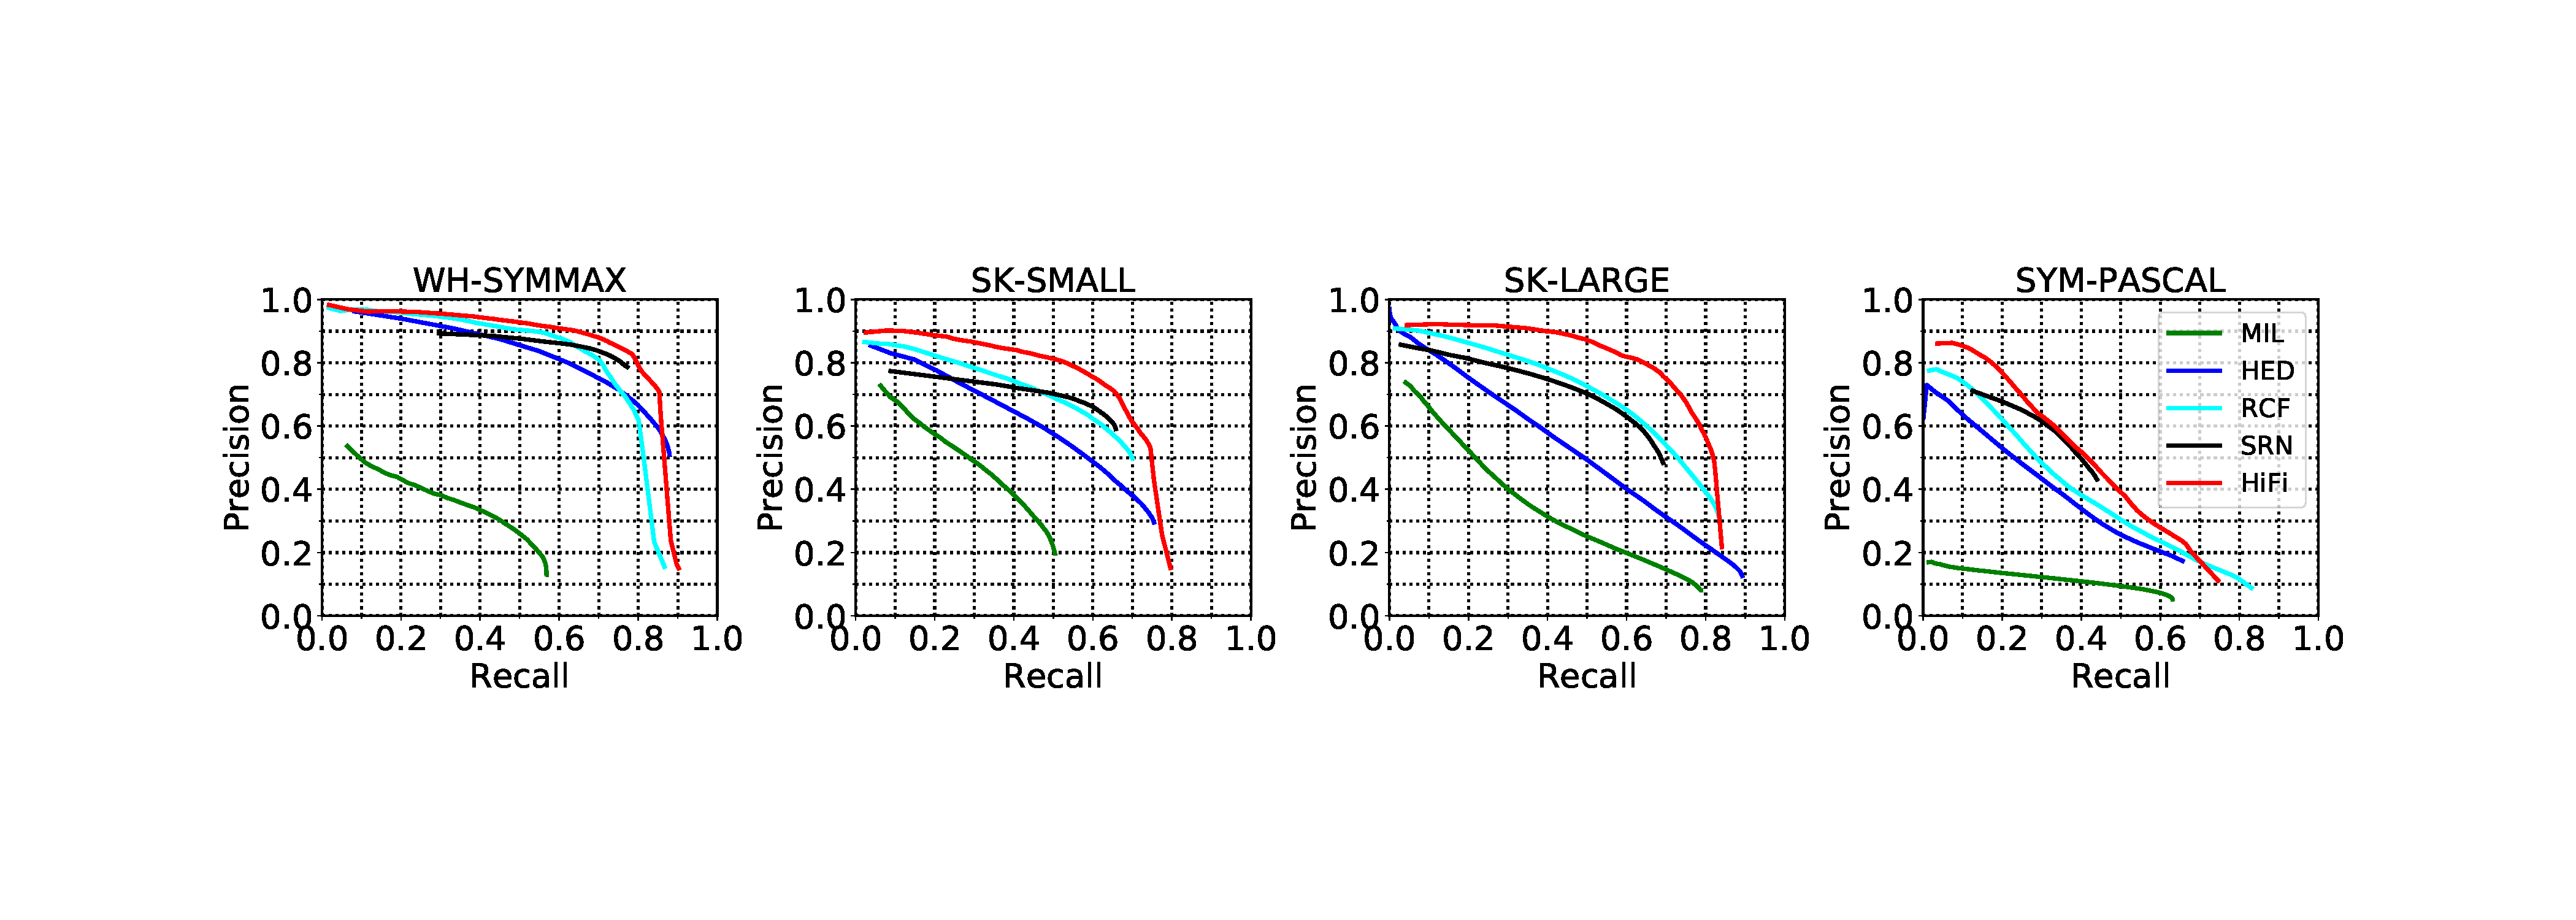
\includegraphics[width=1\linewidth]{figures/pr-curve}
	\caption{一个pdf格式的矢量图。使用\\caption命令为图表添加注解,注解中可以引用参考文献~\cite{shen2017label}。}\label{fig1}
\end{figure}

对于曲线图和柱状图等非照片类图表,我推荐插入pdf格式。pdf格式支持绝大部分主流平台(Windows, Linux, OSX),而且可以方便的自由编辑,文件大小也比较小。
如果你使用Python的Matplotlib画图,那么可以直接用matplotlib.pyplot.savefig()
来导出.pdf格式的图片。
如果你使用Matlab画图的话,只能导出eps格式的矢量图。在\LaTeX中插入eps也没有问题,
但是eps文件比同等条件的pdf稍大,而且不方便编辑。
强迫症患者可以将eps转为pdf后再插入到\LaTeX。

同样是一行四列的布局,图~\ref{fig1}直接插入一个包含四个曲线图的pdf文件,
而图~\ref{fig:fig3d}通过增加一个$1\times4$的表格,然后再每个表格单元中各自插入
一个图标文件。

\begin{figure}[!h]
	\centering
	\begin{overpic}[scale=0.6]{figures/convergence}
		\put(50,41){\large{可使用overpic命令}}
		\put(38, 35){\Large{往图像上覆盖符号$\Sigma$}}
		\put(35,28){\LARGE{公式$f(x)=a\times x$}}
		\put(30,20){\huge{引用公式\ref{eq:cases}。}}
		\put(25,12){\Huge{参考文献\cite{shen2016object}。}}
	\end{overpic}
	\caption{一个pdf格式的矢量图。使用\\caption命令为图表添加注解,注解中可以引用参考文献~\cite{shen2017deepskeleton}。}
	\label{fig3}
\end{figure}

\begin{figure}[!h]
	\centering
	\begin{tabular}{@{}cccc@{}}
		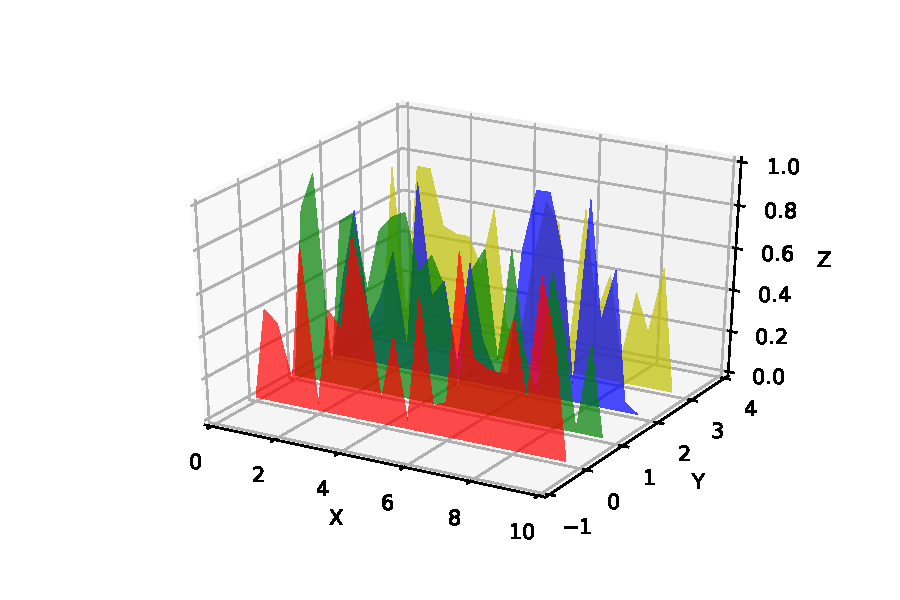
\includegraphics[width=.25\textwidth]{figures/mplot3d}  &
		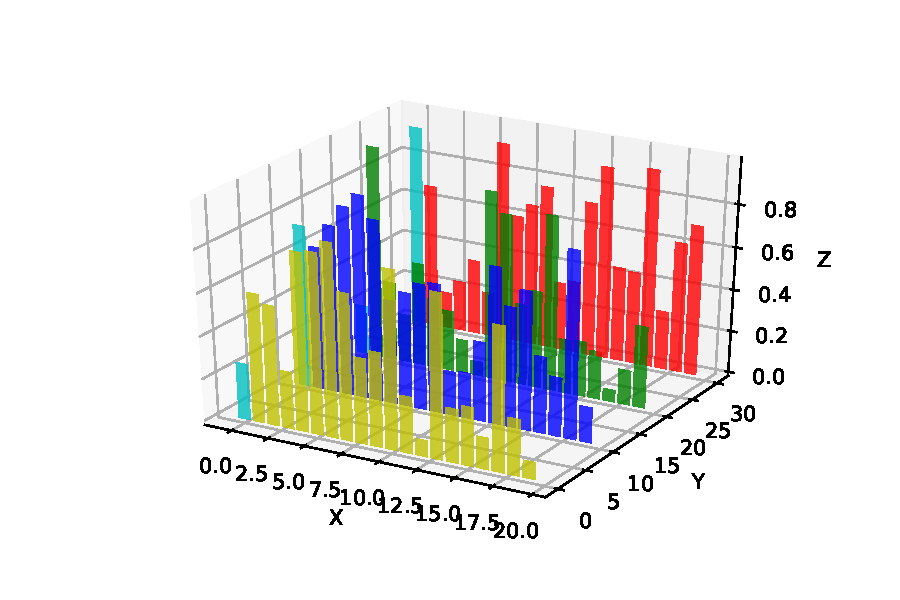
\includegraphics[width=.25\textwidth]{figures/bar3d}  &
		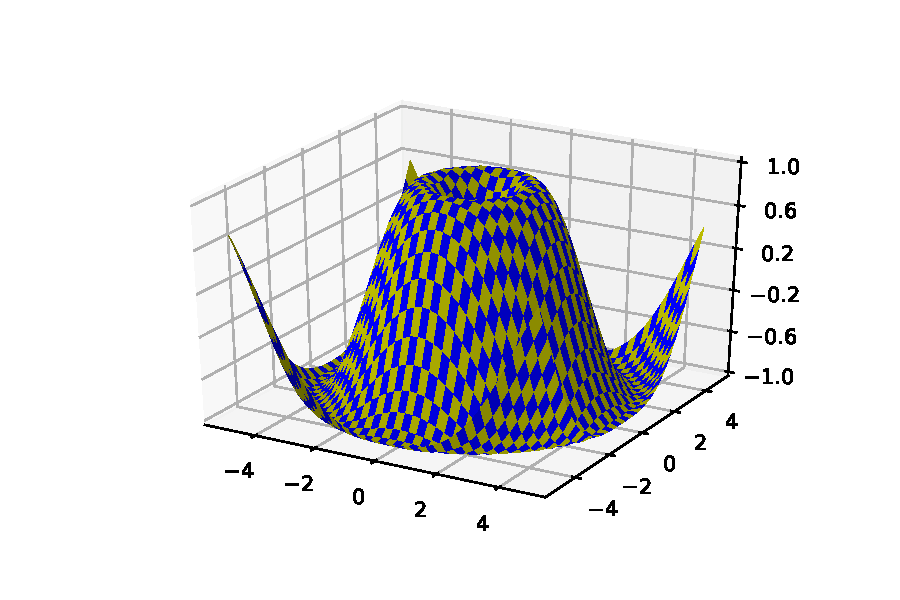
\includegraphics[width=.25\textwidth]{figures/surface3d} &
		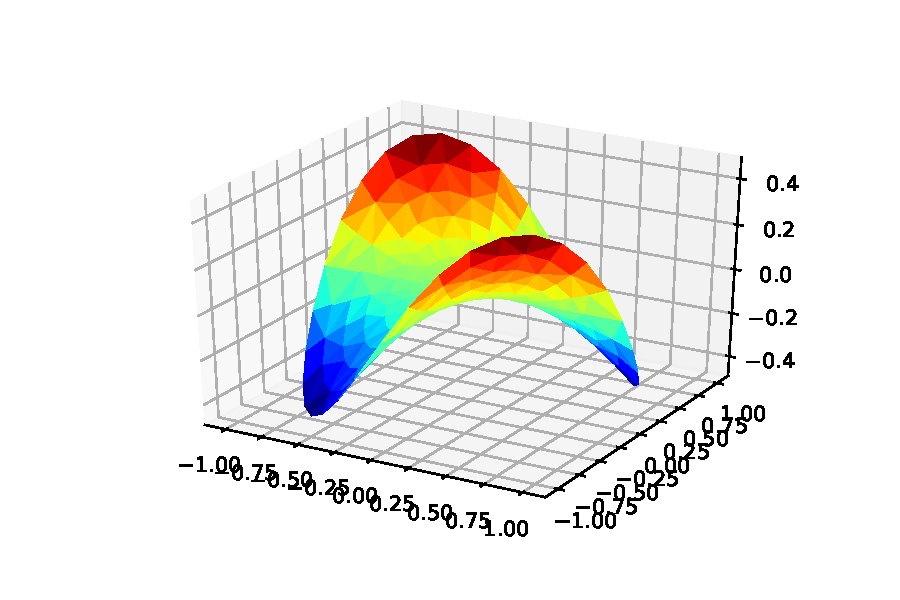
\includegraphics[width=.25\textwidth]{figures/trisurf3d} \\
		(a)M-plot 3D & (b)Bar-chart 3D & 
		(c)Surface 3D & (d) Tri-surface 3D \\
	\end{tabular}
	\caption{通过表格对图片进行布局,在一个$1\times4$表格的每一个单元格中各自插入一个图片文件。
		生成上面四个图对应的Python代码在\href{https://github.com/zeakey/shu-thesis/tree/master/figures}{figures}目录下。}
	\label{fig:fig3d}
\end{figure}
下面是相关代码:
\begin{lstlisting}[captionpos=b,language=Tex]
	\begin{figure}[!h]
		\centering
		\begin{tabular}{@{}cccc@{}}
			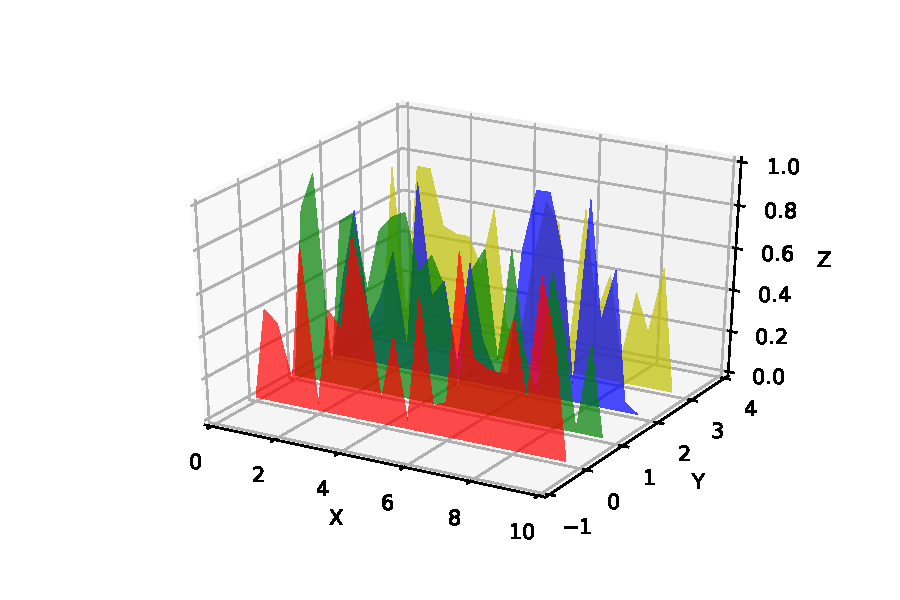
\includegraphics[width=.25\textwidth]{figures/mplot3d}  &
			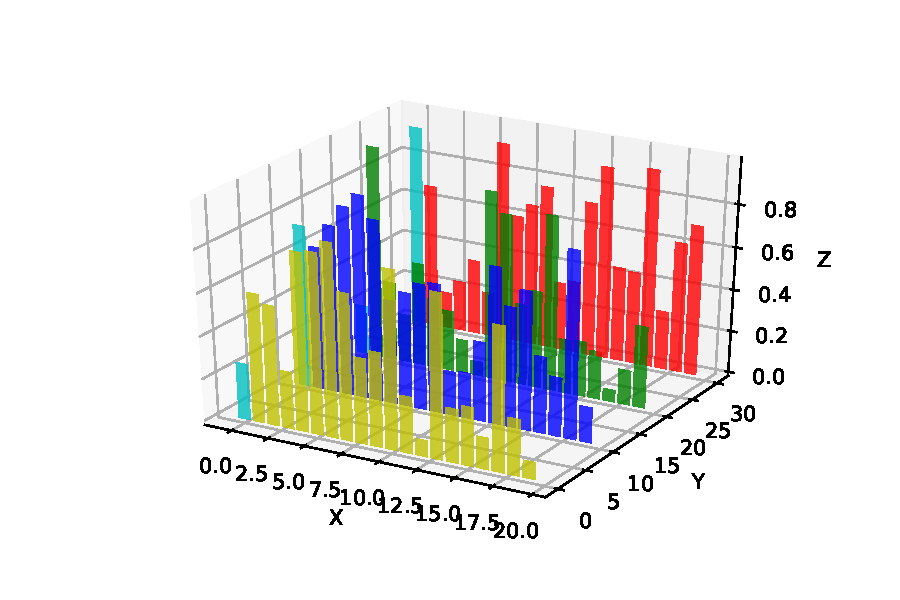
\includegraphics[width=.25\textwidth]{figures/bar3d}  &
			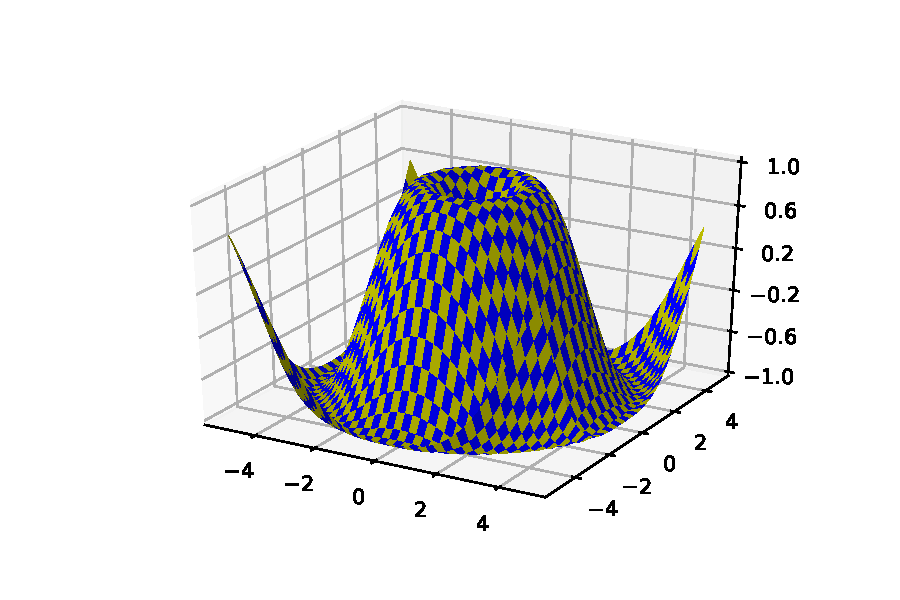
\includegraphics[width=.25\textwidth]{figures/surface3d} &
			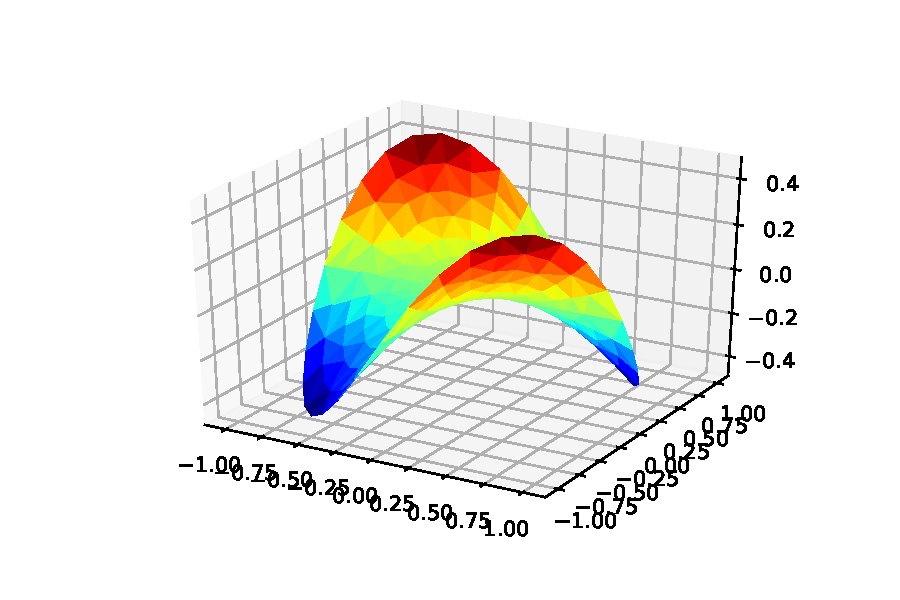
\includegraphics[width=.25\textwidth]{figures/trisurf3d} \\
			(a)M-plot 3D & (b)Bar-chart 3D & 
			(c)Surface 3D & (d) Tri-surface 3D \\
		\end{tabular}
	\end{figure}
\end{lstlisting}

\subsection{绘图}
除了通过直接插入已经生成的图像文件之外,\LaTeX 还可以通过 Tikz 宏包直接绘制函数图像。
%
下面有几个使用Tikz包绘制三位函数曲面和直方图的例子,由于 Tikz 会让编译的时间变长,代码已经被注释。
%
如果你有兴趣的话可以取消注释然后编译查看效果,或者预览预编译的pdf:
\url{http://data.kaiz.xyz/shu-thesis/shu-thesis.pdf}。

%\begin{figure}[!h]
%\centering
%\begin{tabular}{@{}cc@{}}
%  \pgfplotsset{width=0.5\textwidth}
%  \begin{tikzpicture}
	%    \begin{axis}[
		%    hide axis,                              %隐藏坐标
		%    colormap/cool,                          %颜色风格
		%    ]
		%    \addplot3[
		%    mesh,                                   %绘制的三维图像是网格
		%    samples=50,                             %定义域分割数量
		%    domain=-8:8,                            %定义域
		%    ]
		%    {sin(deg(sqrt(x^2+y^2)))/sqrt(x^2+y^2)};    %二元显式函数
		%        \addlegendentry{$\frac{sin(r)}{r}$}         %添加图例
		%    \end{axis}
	%  \end{tikzpicture} & 
%  %==============================%
%  \pgfplotsset{width=0.5\textwidth}
%  \begin{tikzpicture}
	%    \begin{axis}[colorbar]         % 绘制坐标,并设置一个彩色指示条
		%    \addplot3[surf]                % 绘制三维图
		%    {x^2+y^2};                    % 输入二元显式函数
		%    \end{axis}
	%  \end{tikzpicture}
%\end{tabular}
%\caption{通过Tikz绘制函数图像。}
%\label{fig:tikz_surface}
%\end{figure}
%还有直方图:
%\begin{figure}[!hbt]
%\centering
%\pgfplotsset{width=0.5\textwidth}
%\begin{tikzpicture}
%\begin{axis}[ybar,enlargelimits=0.15]  % 绘制关于y坐标的条形图,条形之间的最大间隔是0.15cm
%\addplot[draw=blue,fill=red]           % 蓝色边界、红色填充
%coordinates
%{
	% (0,4) (1,1) (2,2)
	% (3,5) (4,6) (5,1)
	%};
%\addplot[draw=black,fill=blue]         % 黑色边界、蓝色填充
%coordinates
%{
	% (0,3) (1,4) (2,2)
	% (3,9) (4,6) (5,2)
	%};
%\end{axis}
%\end{tikzpicture}
%\caption{通过Tikz绘制直方图。}\label{fig:tikz_hist}
%\end{figure}
%

本章节的所有图像都是\textbf{使用\LaTeX 代码直接绘制的},并没有使用任何Matlab或者matplotlib等第三方程序生成图像。
当然,生成的的图像全部都是矢量图。

%\pagebreak
\subsection{表格}
\LaTeX使用table环境生成表格。下面就是生成表\ref{tab:performance}的\LaTeX代码:

\begin{lstlisting}[captionpos=b,language=Tex]
	\begin{table}[!h]
		\centering
		\setlength\tabcolsep{6.4pt}
		\begin{tabular}{l|c|c|c|c}
			\hline
			\diagbox{Method}{Dataset} & A & B & C & D \\
			\hline
			LMSDS~\cite{shen2017deepskeleton} & 0.365  & 0.392 & 0.293 & 0.174 \\
			LDLF~\cite{shen2017label} & 0.732  & 0.542 & 0.497 & 0.369 \\
			\hline
			\textbf{FSDS} (ours) & 0.769  & 0.623 & 0.633 & 0.418 \\
			\hline
		\end{tabular}\vspace{-6pt}
		\caption{This is a table.}\label{tab:sk-fmeasure}\label{tab:performance}%
	\end{table}%
\end{lstlisting}

\begin{table}[!h]
	\centering
	\setlength\tabcolsep{6.4pt}
	\begin{tabular}{l|c|c|c|c}
		\hline
		\diagbox{Method}{Dataset} & A & B & C & D \\
		\hline
		LMSDS~\cite{shen2017deepskeleton} & 0.365  & 0.392 & 0.293 & 0.174 \\
		LDLF~\cite{shen2017label} & 0.732  & 0.542 & 0.497 & 0.369 \\
		\hline
		\textbf{FSDS} (ours) & 0.769  & 0.623 & 0.633 & 0.418 \\
		\hline
	\end{tabular}\vspace{-6pt}
	\caption{This is a table.}\label{tab:sk-fmeasure}\label{tab:performance}%
\end{table}%

\subsection{图表的排版和定位}\label{sec:location}
\LaTeX相比Word有个缺点就是\emph{非所见即所得}。比如你的两个表格在代码中明明是
相邻一个在前一个在后的,然而排版出来的结果可能是两个被放到了不同的页面中,甚至先后顺序都不对应。
%

\LaTeX图表使用位置参数来确定元素的定位。位置参数有以下几种选项:h (here)、t (top)、b (bottom)、p (我也不知道),分别表示把元素至于当前位置、当前页面的上方、下方。
当你有排版困惑,怎么弄也无法把图标放在自己想要的位置的时候(我经常遇到),最好的解决方法就是疯狂前后移动图表元素对应代码,总有一个位置会是对的。
%
\href{https://tex.stackexchange.com/questions/35125/how-to-use-the-placement-options-t-h-with-figures}{这里}是一个对位置参数的详细介绍。


\pagebreak
% !TeX spellcheck = <none>
\section{交叉引用}\label{sec:ref}
%%%%%%%%%%%%%%%%%%%%%%%%%%%%%%%%%%%%%%%%%%%%%%%%%%%%%%%
交叉引用可以说是\LaTeX的核心竞争力了。
我们经常需要在论文中引用文献和文章中的图表,比如说:“根据文献
~\cite{shen2017label},~\cite{shen2016object}和~\cite{shen2017deepskeleton}
所描述的的方法,
以式\ref{eq:cases}作为评价标准,我们可以得到如图~\ref{fig1}所示的性能曲线以及
表~\ref{tab:sk-fmeasure}中的定量型能比较。从图~\ref{fig1}和表~\ref{tab:sk-fmeasure}的结果来看,~\cite{shen2016object}和~\cite{shen2017deepskeleton}
具有较好的检测效果”。

如果你使用Word撰写学位论文,可以想象一下情景:你的论文有50+条引用,
你要在论文中反复交叉引用这些参考文献;然后现在你发现你的绪论部分需要补充一条
参考文献,而有的引用格式要求参考文献引用标号按文中出现先后的顺序排列,
当插入一条参考文献之后你如何处理后续的参考文献编号?
%%


或者有下面一个场景:当你完成第三章写作之后发现图3.6和图3.7之间要再插入一张图,然后
你发现图3.7和图3.7之后的所有图片的标号都要改,而且你的文中所有引用到这些图的地方都需要修改。

\textbf{\LaTeX强大的交叉引用功能}将把你从繁琐的文献/图表/公式标号中解放出来,
你只用关注写作本身,其他的事情会帮你自动完成。
%
当你写完一个图表/公式,给它添加一个label属性,然后在需要引用的地方使用ref\{the-label\}
进行引用,\LaTeX将自动为你排好序号。
%
比如"根据文献~\cite{shen2017label},~\cite{shen2016object}
和~\cite{shen2017deepskeleton}所描述的的方法,
以式\ref{eq:matrix}作为评价标准,我们可以得到如图~\ref{fig1}所示的性能曲线以及
表~\ref{tab:sk-fmeasure}中的定量型能比较。从图~\ref{fig1}和表~\ref{tab:sk-fmeasure}的结果来看,~\cite{shen2016object}和~\cite{shen2017deepskeleton}
具有较好的检测效果"。

\TeX文档中的所有内容都可以添加label属性从而进行交叉引用。比如说文章的一个子章节
(subsection)就可以被引用:第\ref{sec:location}章描述了如何对\TeX元素进行定位。

更强大的是,所有的生成的引用标号都是可以点击的,
当你在生成的pdf中点击引用标号,将自动弹到对应的文献/图表/公式处。
%
另外,在文章最后的参考文献列表中,每一条参考文献的末尾都会标注这条参考文献在哪一页被引用。

%

\pagebreak
%%%%%%%%%%%%%%%%%%%%%%%%%%%%%%%%%%%%%%%%%%%%%%%%%%%%%%%
\section{有用的链接}
%%%%%%%%%%%%%%%%%%%%%%%%%%%%%%%%%%%%%%%%%%%%%%%%%%%%%%%
\begin{itemize}
	\item 数学符号速查表 \url{http://web.ift.uib.no/Teori/KURS/WRK/TeX/symALL.html}
	\item 字体大小 \url{https://texblog.org/2012/08/29/changing-the-font-size-in-latex/}
	\item 一个比较全的 \LaTeX \ WiKi \url{https://en.wikibooks.org/wiki/LaTeX}
\end{itemize}

\pagebreak
%%%%%%%%%%%%%%%%%%%%%%%%%%%%%%%%%%%%%%%%%%%%%%%%%%%%%%%
\section{参考文献}
%%%%%%%%%%%%%%%%%%%%%%%%%%%%%%%%%%%%%%%%%%%%%%%%%%%%%%%
\LaTeX使用bib(或者latexbib)管理参考文献。新增参考文献条目时只需要在将bib格式的参考文献加入bib文件中,然后重新编译即可。在文中使用cite\{citationA\}引用即可。
点击参考文献编号\cite{shen2017deepskeleton}可跳转至对应的参考文献条目。

%\begin{comment}
% 插图索引表
\pagebreak
\addcontentsline{toc}{section}{插图索引}
\listoffigures
\pagebreak
\addcontentsline{toc}{section}{表格索引}
\listoftables

%\begin{comment}
%% 参考文献
\pagebreak
\addcontentsline{toc}{section}{参考文献}
%\bibliography{master-thesis} % bibtex 要求的指定文献可文件的方式 会默认在这里打印参考文献列表,biblatex要求这个命令只能在导言区出现
% bibintoc就表示会在目录中加参考文献
\printbibliography[] % biblatex 打印文献列表的方式

%%%%%%%%%%%%%%%%%%%%%%%%%%%%%%%%%%%%%%%%%%%%%%%%%%%%%%%%%%%%%%%%%%%%%%%%%%%%%%%%%%%
%%%%%%%%%%%%%%%%%%%%%%%%%%%%%%%%%%%%%%%%%%%%%%%%%%%%%%%%%%%%%%%%%%%%%%%%%%%%%%%%%%%
\pagebreak

\section*{作者在攻读专业硕士学位期间取得的研究成果}
\addcontentsline{toc}{section}{作者在攻读专业硕士学位期间取得的研究成果}

%学硕请自行替换标题名

\noindent
\textbf{一、 论文}

[1] xxx

[2] xxx

\noindent
\textbf{二、项目}

[1] xxx

[2] xxx

\noindent	
\textbf{三、软著}

[1] xxx

[2] xxx



%%%%%%%%%%%%%%%%%%%%%%%%%%%%%%%%%%%%%%%%%%%%%%%%%%%%%%%%%%%%%%%%%%%%%%%%%%%%%%%%%%%
%%%%%%%%%%%%%%%%%%%%%%%%%%%%%%%%%%%%%%%%%%%%%%%%%%%%%%%%%%%%%%%%%%%%%%%%%%%%%%%%%%%

\pagebreak

\section*{致\hspace{\ccwd}谢}
\addcontentsline{toc}{section}{致谢}

感谢。。。。。。

\rightline{作者}

\rightline{地点}

\rightline{时间}


\end{document}
